%!TEX root = ../main.tex

\section{Results}
\label{s:results}
In this section we present our results. \Crefs{s:results:normals} compares the computational complexity of the computation of the `real' and `fake' normals. Furthermore it contrasts the visual results. \Crefs{s:results:pipeline} compares the results of the implementation by \citeauthor{vlachos2001curved} on the CPU with our implementation on the GPU.

%!TEX root = ../main.tex
\subsection{Fake versus real normals}
\label{s:results:normals}
	\todo[inline]{Show results of PN triangles with fake and real normals, and discuss differences}
	\todo[inline]{Computational complexity of the fake normals and the real normals, consider one triangle.}
	\todo[inline]{Any unsolved problems?}

\iftoggle{PHONG}{
	\subsection{Phong tesselation versus PN triangles}
	\future{Show comparison of Phong tesselation with PN triangles: performance, visual results, continuity, probably in cooperation with Jelle and Gerben}
	\future{Any unsolved problems?}
}

%!TEX root = ../main.tex

\subsection{Pipeline}
\label{s:results:pipeline}
	\Cref{fig:results:cpugpu} shows the rendering by \citeauthor{vlachos2001curved} next to our rendering of, probably, the same model. The only difference between these two models should be the pattern in which the triangles of the input mesh are subdivided into flat triangles. A visual inspection shows no obvious differences between the models, leading us to suggest that the difference in triangulation does not matter much. 

	%!TEX root = ../main.tex
\begin{figure*}
	\centering
	\begin{subfigure}[b]{0.2\textwidth}
		\centering
		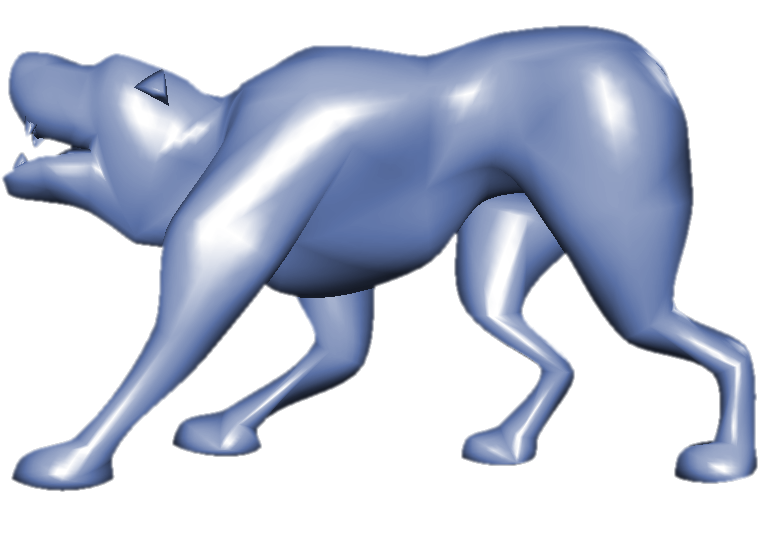
\includegraphics[width=\textwidth]{content/img/results/cpugpu/dogCPU.png}
		\caption{Rottweiler on CPU}
		\label{fig:results:cpugpu:cpuDog}
	\end{subfigure}
	\hspace{0.1\textwidth}
	\begin{subfigure}[b]{0.2\textwidth}
		\centering
		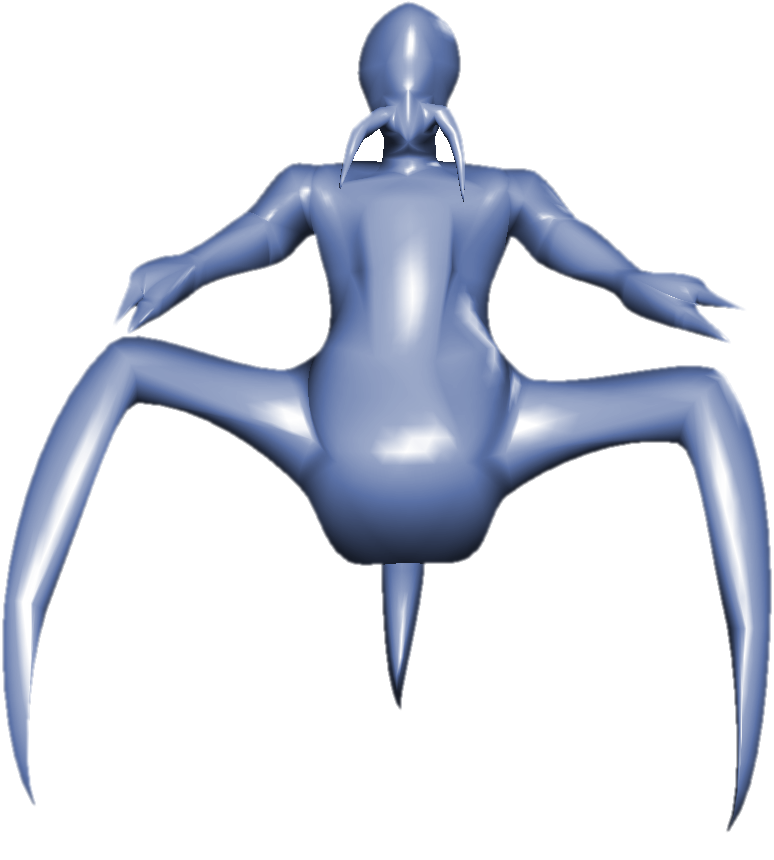
\includegraphics[width=\textwidth]{content/img/results/cpugpu/voreCPU.png}
		\caption{Vore on CPU}
		\label{fig:results:cpugpu:cpuVore}
	\end{subfigure}	
	\hspace{0.1\textwidth}
	\begin{subfigure}[b]{0.2\textwidth}
		\centering
		\includegraphics[width=\textwidth]{content/img/results/cpugpu/shamblercpu.png}
		\caption{Shambler on CPU}
		\label{fig:results:cpugpu:cpuShambler}
	\end{subfigure}		

	\begin{subfigure}[b]{0.2\textwidth}
		\centering
		\includegraphics[width=\textwidth]{content/img/results/cpugpu/doggpu.png}
		\caption{Rottweiler on GPU}
		\label{fig:results:cpugpu:gpuDog}
	\end{subfigure}
	\hspace{0.1\textwidth}
	\begin{subfigure}[b]{0.2\textwidth}
		\centering
		\includegraphics[width=\textwidth]{content/img/results/cpugpu/voregpu.png}
		\caption{Vore on GPU}
		\label{fig:results:cpugpu:gpuVore}
	\end{subfigure}	
	\hspace{0.1\textwidth}
	\begin{subfigure}[b]{0.2\textwidth}
		\centering
		
\includegraphics[width=\textwidth]{content/img/results/cpugpu/shamblerGPU.png}
		\caption{Shambler on GPU}
		\label{fig:results:cpugpu:gpuShambler}
	\end{subfigure}			
	\caption{A family of game characters from the game Quake 1. \Cref{fig:results:cpugpu:cpuDog,fig:results:cpugpu:cpuVore,fig:results:cpugpu:cpuShambler} are rendered on a CPU by \citeauthor{vlachos2001curved}. \Cref{fig:results:cpugpu:gpuDog,fig:results:cpugpu:gpuVore,fig:results:cpugpu:gpuShambler} are rendered by our implementation. We rendered our models with the Phong shading and reflection model ($k_s = 0.3$, $k_d = 0.5$, $k_a = 0.4$, $\alpha = 150.0$, color = $(0.988, 0.0, 0.427)$), with a single light source $\left(I_s = I_d = I_a = (1.0, 1.0, 1.0)\right)$ at $(-2.0, 5.0, -10.0)$. The inner and outer tessellation levels were set to $12.0$. The eye was placed at $(2.0, 5.0, -10.0)$.
% 
	\Cref{fig:results:cpugpu:cpuDog,fig:results:cpugpu:cpuVore,fig:results:cpugpu:cpuShambler} were taken from \textcite{vlachos2001curved}.}
	\label{fig:results:cpugpu}
\end{figure*}